\normaltrue
\correctionfalse

%\UPSTIidClasse{11} % 11 sup, 12 spé
%\newcommand{\UPSTIidClasse}{12}

\exer{Mouvement RT  $\star$ \label{B2:13:PTSI:06:02}}
\setcounter{question}{0}\UPSTIcompetence{B2-13}
\index{Compétence B2-13-PTSI}
\index{Mécanisme à 1 translation et 1 rotation}
\ifcorrection
\else
\marginnote{\textbf{Pas de corrigé pour cet exercice.}}
\fi

\ifprof
\else
Soit le mécanisme suivant. 
\begin{center}
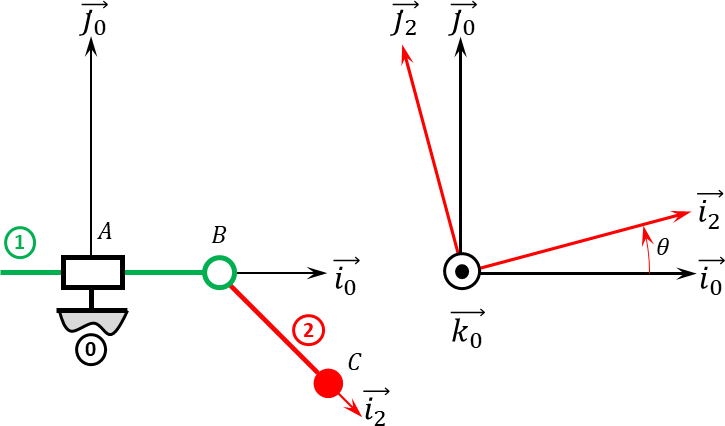
\includegraphics[width=\linewidth]{06_TR_01}
\end{center}
\fi

\question{Réaliser le paramétrage du mécanisme.}
\ifprof ~\\

\else
\fi

\ifprof
\else
\footnotesize

\normalsize
\begin{flushright}
\footnotesize{Corrigé  voir \ref{B2:13:PTSI:06:02}.}
\end{flushright}%
\fi